\documentclass{standalone}
\usepackage{tikz}
\usetikzlibrary{patterns, positioning}


\begin{document}
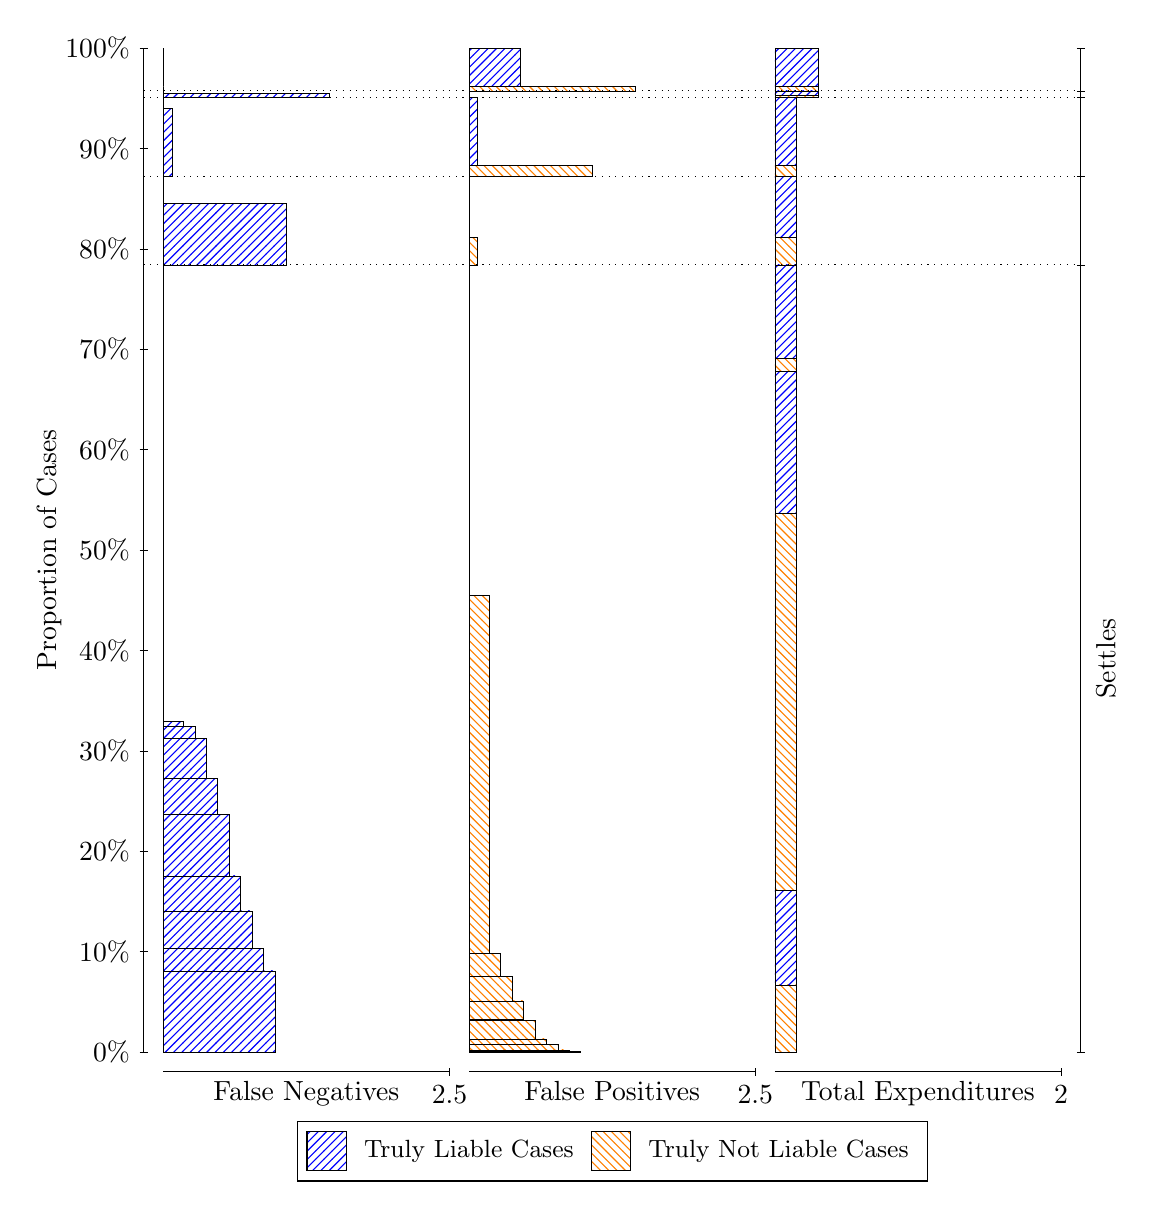
\begin{tikzpicture}
\draw[black, very thin] (1.5,1.75) -- (1.5,14.5);
\node[rotate=90, text=black, anchor=center] at (0.3, 8.125) {Proportion of Cases};
\draw[black, very thin] (1.45,1.75) -- (1.55,1.75);
\node[text=black, anchor=east] at (1.45, 1.75) {0\%};
\draw[black, very thin] (1.45,3.025) -- (1.55,3.025);
\node[text=black, anchor=east] at (1.45, 3.025) {10\%};
\draw[black, very thin] (1.45,4.3) -- (1.55,4.3);
\node[text=black, anchor=east] at (1.45, 4.3) {20\%};
\draw[black, very thin] (1.45,5.575) -- (1.55,5.575);
\node[text=black, anchor=east] at (1.45, 5.575) {30\%};
\draw[black, very thin] (1.45,6.85) -- (1.55,6.85);
\node[text=black, anchor=east] at (1.45, 6.85) {40\%};
\draw[black, very thin] (1.45,8.125) -- (1.55,8.125);
\node[text=black, anchor=east] at (1.45, 8.125) {50\%};
\draw[black, very thin] (1.45,9.4) -- (1.55,9.4);
\node[text=black, anchor=east] at (1.45, 9.4) {60\%};
\draw[black, very thin] (1.45,10.675) -- (1.55,10.675);
\node[text=black, anchor=east] at (1.45, 10.675) {70\%};
\draw[black, very thin] (1.45,11.95) -- (1.55,11.95);
\node[text=black, anchor=east] at (1.45, 11.95) {80\%};
\draw[black, very thin] (1.45,13.225) -- (1.55,13.225);
\node[text=black, anchor=east] at (1.45, 13.225) {90\%};
\draw[black, very thin] (1.45,14.5) -- (1.55,14.5);
\node[text=black, anchor=east] at (1.45, 14.5) {100\%};

\draw[black, very thin] (13.4,1.75) -- (13.4,14.5);
\draw[black, very thin] (13.35,1.75) -- (13.45,1.75);
\node[anchor=west] at (13.35, 1.75) {};
\draw[black, very thin] (13.35,11.746) -- (13.45,11.746);
\node[anchor=west] at (13.35, 11.746) {};
\draw[black, very thin] (13.35,12.872) -- (13.45,12.872);
\node[anchor=west] at (13.35, 12.872) {};
\draw[black, very thin] (13.35,13.871) -- (13.45,13.871);
\node[anchor=west] at (13.35, 13.871) {};
\draw[black, very thin] (13.35,13.957) -- (13.45,13.957);
\node[anchor=west] at (13.35, 13.957) {};
\draw[black, very thin] (13.35,14.5) -- (13.45,14.5);
\node[anchor=west] at (13.35, 14.5) {};

\draw[black, very thin, pattern color=blue, pattern=north east lines] (1.75,1.75) rectangle (3.167,2.7812);
\draw[black, very thin, pattern color=blue, pattern=north east lines] (1.75,2.7812) rectangle (3.0217,3.0614);
\draw[black, very thin, pattern color=blue, pattern=north east lines] (1.75,3.0614) rectangle (2.8763,3.5427);
\draw[black, very thin, pattern color=blue, pattern=north east lines] (1.75,3.5427) rectangle (2.731,3.9859);
\draw[black, very thin, pattern color=blue, pattern=north east lines] (1.75,3.9859) rectangle (2.5857,4.7639);
\draw[black, very thin, pattern color=blue, pattern=north east lines] (1.75,4.7639) rectangle (2.4403,5.2223);
\draw[black, very thin, pattern color=blue, pattern=north east lines] (1.75,5.2223) rectangle (2.295,5.7324);
\draw[black, very thin, pattern color=blue, pattern=north east lines] (1.75,5.7324) rectangle (2.1497,5.8826);
\draw[black, very thin, pattern color=blue, pattern=north east lines] (1.75,5.8826) rectangle (2.0043,5.9476);
\draw[black, very thin, pattern color=orange, pattern=north west lines] (1.75,5.9476) rectangle (1.75,11.746);
\draw[black, very thin, pattern color=blue, pattern=north east lines] (1.75,11.746) rectangle (3.3123,12.526);
\draw[black, very thin, pattern color=orange, pattern=north west lines] (1.75,12.526) rectangle (1.75,12.872);
\draw[black, very thin, pattern color=blue, pattern=north east lines] (1.75,12.872) rectangle (1.859,13.729);
\draw[black, very thin, pattern color=orange, pattern=north west lines] (1.75,13.729) rectangle (1.75,13.871);
\draw[black, very thin, pattern color=blue, pattern=north east lines] (1.75,13.871) rectangle (3.8573,13.926);
\draw[black, very thin, pattern color=orange, pattern=north west lines] (1.75,13.926) rectangle (1.75,13.957);
\draw[black, very thin, pattern color=orange, pattern=north west lines] (1.75,13.957) rectangle (1.75,14.014);
\draw[black, very thin, pattern color=blue, pattern=north east lines] (1.75,14.014) rectangle (1.75,14.5);
\draw[black, very thin, pattern color=orange, pattern=north west lines] (5.6333,1.75) rectangle (7.0503,1.7563);
\draw[black, very thin, pattern color=orange, pattern=north west lines] (5.6333,1.7563) rectangle (6.905,1.7776);
\draw[black, very thin, pattern color=orange, pattern=north west lines] (5.6333,1.7776) rectangle (6.7597,1.8493);
\draw[black, very thin, pattern color=orange, pattern=north west lines] (5.6333,1.8493) rectangle (6.6143,1.9158);
\draw[black, very thin, pattern color=orange, pattern=north west lines] (5.6333,1.9158) rectangle (6.469,2.1475);
\draw[black, very thin, pattern color=orange, pattern=north west lines] (5.6333,2.1475) rectangle (6.3237,2.1678);
\draw[black, very thin, pattern color=orange, pattern=north west lines] (5.6333,2.1678) rectangle (6.3237,2.3996);
\draw[black, very thin, pattern color=orange, pattern=north west lines] (5.6333,2.3996) rectangle (6.1783,2.712);
\draw[black, very thin, pattern color=orange, pattern=north west lines] (5.6333,2.712) rectangle (6.033,2.9984);
\draw[black, very thin, pattern color=orange, pattern=north west lines] (5.6333,2.9984) rectangle (5.8877,7.5485);
\draw[black, very thin, pattern color=blue, pattern=north east lines] (5.6333,7.5485) rectangle (5.6333,11.746);
\draw[black, very thin, pattern color=orange, pattern=north west lines] (5.6333,11.746) rectangle (5.7423,12.092);
\draw[black, very thin, pattern color=blue, pattern=north east lines] (5.6333,12.092) rectangle (5.6333,12.872);
\draw[black, very thin, pattern color=orange, pattern=north west lines] (5.6333,12.872) rectangle (7.1957,13.014);
\draw[black, very thin, pattern color=blue, pattern=north east lines] (5.6333,13.014) rectangle (5.7423,13.871);
\draw[black, very thin, pattern color=orange, pattern=north west lines] (5.6333,13.871) rectangle (5.6333,13.902);
\draw[black, very thin, pattern color=blue, pattern=north east lines] (5.6333,13.902) rectangle (5.6333,13.957);
\draw[black, very thin, pattern color=orange, pattern=north west lines] (5.6333,13.957) rectangle (7.7407,14.014);
\draw[black, very thin, pattern color=blue, pattern=north east lines] (5.6333,14.014) rectangle (6.2873,14.5);
\draw[black, very thin, pattern color=orange, pattern=north west lines] (9.5167,1.75) rectangle (9.7892,2.6009);
\draw[black, very thin, pattern color=blue, pattern=north east lines] (9.5167,2.6009) rectangle (9.7892,3.8056);
\draw[black, very thin, pattern color=orange, pattern=north west lines] (9.5167,3.8056) rectangle (9.7892,8.5874);
\draw[black, very thin, pattern color=blue, pattern=north east lines] (9.5167,8.5874) rectangle (9.7892,10.397);
\draw[black, very thin, pattern color=orange, pattern=north west lines] (9.5167,10.397) rectangle (9.7892,10.562);
\draw[black, very thin, pattern color=blue, pattern=north east lines] (9.5167,10.562) rectangle (9.7892,11.746);
\draw[black, very thin, pattern color=orange, pattern=north west lines] (9.5167,11.746) rectangle (9.7892,12.092);
\draw[black, very thin, pattern color=blue, pattern=north east lines] (9.5167,12.092) rectangle (9.7892,12.872);
\draw[black, very thin, pattern color=orange, pattern=north west lines] (9.5167,12.872) rectangle (9.7892,13.014);
\draw[black, very thin, pattern color=blue, pattern=north east lines] (9.5167,13.014) rectangle (9.7892,13.871);
\draw[black, very thin, pattern color=orange, pattern=north west lines] (9.5167,13.871) rectangle (10.062,13.902);
\draw[black, very thin, pattern color=blue, pattern=north east lines] (9.5167,13.902) rectangle (10.062,13.957);
\draw[black, very thin, pattern color=orange, pattern=north west lines] (9.5167,13.957) rectangle (10.062,14.014);
\draw[black, very thin, pattern color=blue, pattern=north east lines] (9.5167,14.014) rectangle (10.062,14.5);
\draw[black, dotted] (1.5,11.746) -- (13.4,11.746);
\draw[black, dotted] (1.5,12.872) -- (13.4,12.872);
\draw[black, dotted] (1.5,13.871) -- (13.4,13.871);
\draw[black, dotted] (1.5,13.957) -- (13.4,13.957);
\draw[black, very thin] (1.75,1.5) -- (5.3833,1.5);
\node[text=black, anchor=north] at (3.5667, 1.5) {False Negatives};
\draw[black, very thin] (5.3833,1.45) -- (5.3833,1.55);
\node[text=black, anchor=north] at (5.3833, 1.45) {2.5};

\draw[black, very thin] (5.6333,1.5) -- (9.2667,1.5);
\node[text=black, anchor=north] at (7.45, 1.5) {False Positives};
\draw[black, very thin] (9.2667,1.45) -- (9.2667,1.55);
\node[text=black, anchor=north] at (9.2667, 1.45) {2.5};

\draw[black, very thin] (9.5167,1.5) -- (13.15,1.5);
\node[text=black, anchor=north] at (11.333, 1.5) {Total Expenditures};
\draw[black, very thin] (13.15,1.45) -- (13.15,1.55);
\node[text=black, anchor=north] at (13.15, 1.45) {2};

\node[text=black, centered, rotate=90] at (13.72, 6.7481) {Settles};





\draw (7.449999999999999,1.5) node[draw=none] (baseCoordinate) {};
\begin{scope}[align=center]
        \matrix[scale=0.5, draw=black, below=0.5cm of baseCoordinate, nodes={draw}, column sep=0.1cm]{
            \node[rectangle, draw, minimum width=0.5cm, minimum height=0.5cm, pattern color=blue, pattern=north east lines] {}; &
            \node[draw=none, font=\small, text=black] (B) {Truly Liable Cases}; &
            \node[rectangle, draw, minimum width=0.5cm, minimum height=0.5cm, pattern color=orange, pattern=north west lines] {}; &
            \node[draw=none, font=\small, text=black] (B) {Truly Not Liable Cases}; \\
            };
\end{scope}

\end{tikzpicture}
\end{document}